\documentclass{beamer}
\usepackage{preamble_beamer}

\newtheorem*{question*}{Вопрос}
\newtheorem*{claim*}{Утверждение}

\newcommand{\vanilla}{\ensuremath{\mathrm{vanilla}}}
\newcommand{\option}{\ensuremath{\mathrm{option}}}
\newcommand{\payoff}{\ensuremath{\mathrm{payoff}}}
\newcommand{\strike}{\ensuremath{\mathrm{strike}}}
\newcommand{\cashflow}{\ensuremath{\mathrm{cashflow}}}
\newcommand{\fee}{\ensuremath{\mathrm{fee}}}
\newcommand{\exposure}{\ensuremath{\mathrm{exposure}}}
% \newcommand{\condexpec}[1]{\mathbb{E}\left(#1\;\big|\;#2\right)}
\newcommand{\eps}{\varepsilon}  % нормальная буква эпсилон
\newcommand{\red}[1]{\textcolor{red}{#1}}
\newcommand{\blue}[1]{\textcolor{blue}{#1}}
\newcommand{\green}[1]{\textcolor{green}{#1}}
\newcommand{\orange}[1]{\textcolor{orange}{#1}}

\newcommand*{\QEDB}{\null\nobreak\hfill\ensuremath{\square}}

\title[Модели стохастической волатильности]{Лекция 10. Локальная волатильность} % The short title appears at the bottom of every slide, the full title is only on the title page

\begin{document}

\begin{frame}
\titlepage 
\end{frame}

\begin{frame}{Модель Блэка-Шоулза}
    Основные предположения:
    \begin{itemize}
        \item Лог-доходности независимы и имеют нормальное распределение
        \item Параметры модели (ставка и волатильность) постоянные или зависят только от времени.
        \item Можно брать кредиты/класть на счёт деньги под одну и ту же ставку $r$
        \item Нет кредитного риска
        \item Непрерывная торговля, без комиссий и market impact
    \end{itemize}
\end{frame}

\begin{frame}{Исторические доходности}
    \begin{itemize}
        \item Определим лог-доходности для реального процесса и геометрического броуновского движения:
        $$
            L_t = \ln \dfrac{S_t}{S_{t-\delta}}
        $$
        \item Визуально очень отличаются:
    \end{itemize}
\begin{figure}
    \centering
    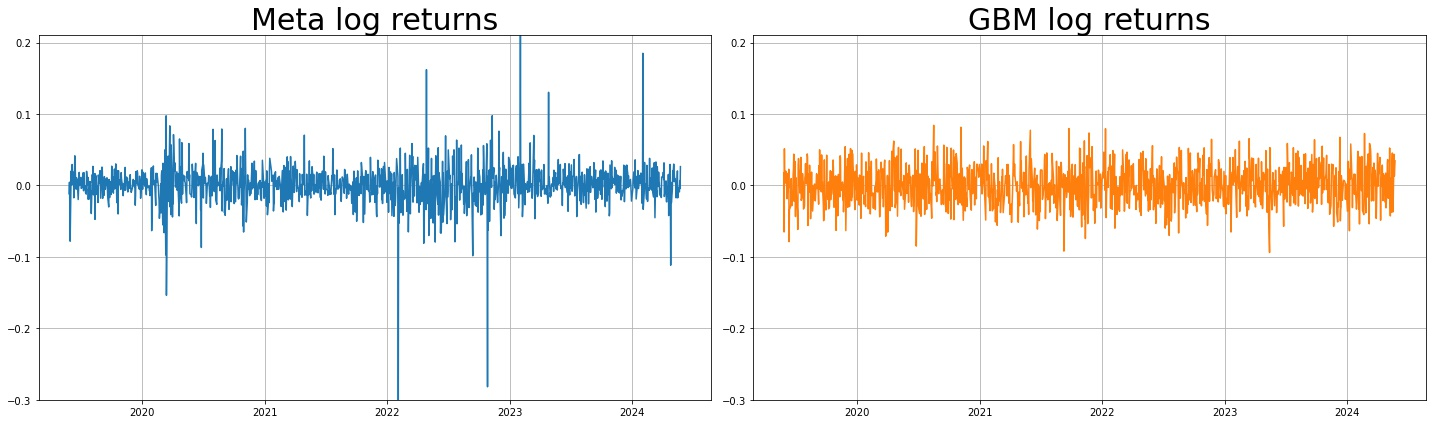
\includegraphics[width=1\linewidth]{10_figs/Meta Log returns plot.jpg}
    \label{fig:enter-label}
\end{figure}
\end{frame}
\begin{frame}{Исторические доходности}
    \begin{itemize}
        \item Исторические доходности имеют толстые хвосты
        \item Коэффициент эксцесса(kurtosis):
            $$
                \kappa = \dfrac{\mathbb{E}\left(L_t-\mathbb{E} L_t\right)^4}{\sigma^4} - 3
            $$
        \item Для нормального $\kappa = 0$, для историчесских данных $\hat{\kappa} \approx 23$. 
    \end{itemize}
    \begin{figure}
    \centering
    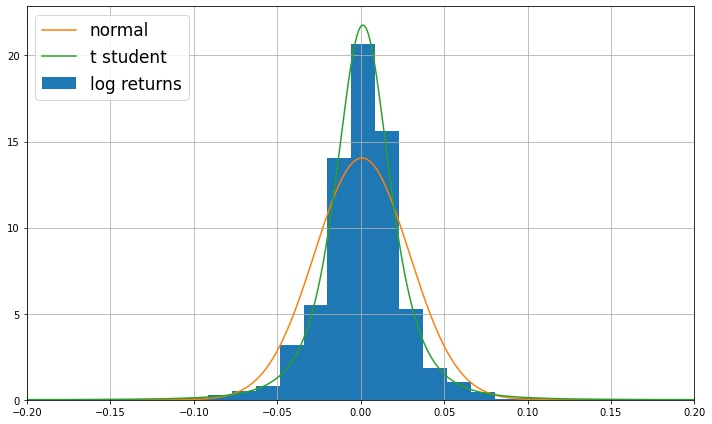
\includegraphics[width=0.8\linewidth]{10_figs/Meta Log returns hist.jpg}
    \label{fig:enter-label}
\end{figure}
\end{frame}

\begin{frame}{Исторические доходности}
    \begin{itemize}
        \item Для геометрического броуновского движения:
        $$
            L_t \perp L_{t + s}, \; \forall s \geq \Delta t
        $$
        \item Для рыночных данных:
        $$
            \mathrm{cov}(L_t, L_{t+s}) \approx 0, \;
            \mathrm{cov}(|L_t|, |L_{t+s}|) \neq 0
        $$ 
    \end{itemize}
    \begin{figure}
    \centering
    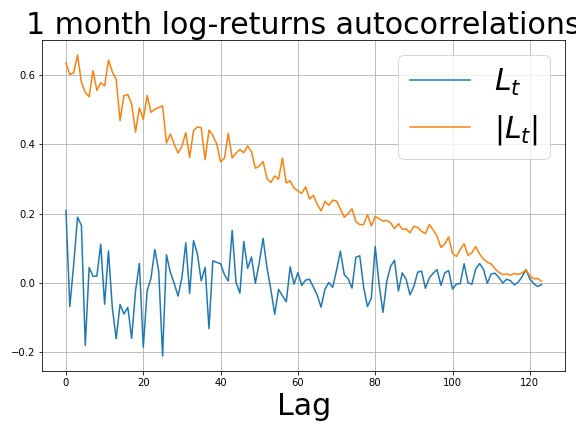
\includegraphics[width=0.65\linewidth]{10_figs/autocorrelation.jpg}
    \label{fig:enter-label}
\end{figure}
\end{frame}

\begin{frame}{Другие стилизованные факты}
    \begin{itemize}
        \item Корреляция между волатильностью и ценой
        \item Кластеризация волатильности
        \item Прыжки в доходностях
    \end{itemize}
\end{frame}

\begin{frame}{Вменяемая волатильность}
    \begin{itemize}
        \item Формула Блэка-Шоулза:
        $$
            V_{BS}(S, T, K, r, \sigma) = S \Phi(d_1) - e^{-rT} K \Phi(d_2)
        $$
        \item Знаем рыночные цены $V_{market}$, можем решить уравнение относительно $\sigma_{implied}$:
        $$
            V_{BS}(S, T, K, r, \sigma_{implied}) = V_{market}
        $$
        \item В модели Блэка-Шоулза $\sigma_{implied} = \sigma$ -- постоянная. На практике $\sigma_{implied} = \sigma_{implied}(T, K)$.
    \end{itemize}
\end{frame}

\begin{frame}{Вменяемая волатильность}
    \begin{figure}
    \centering
    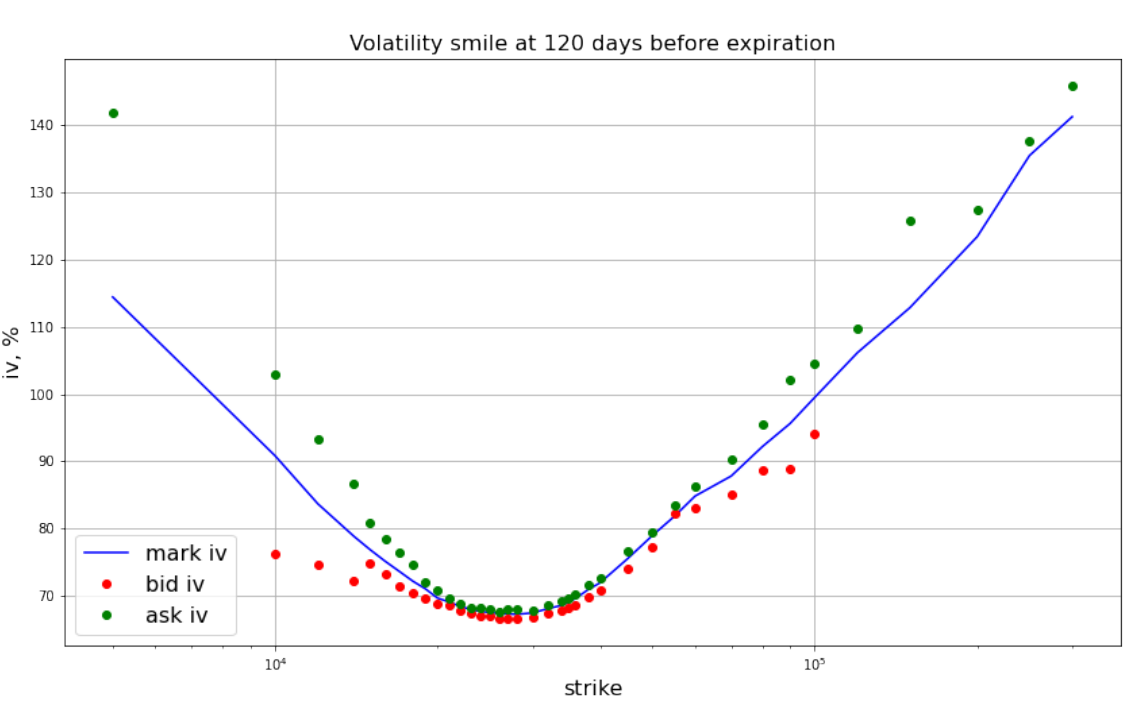
\includegraphics[width=1.05\linewidth]{10_figs/vol smile btc.png}
    \label{fig:enter-label}
\end{figure}
\end{frame}

\begin{frame}{Вменяемая волатильность}
    \begin{itemize}
        \item Как считать $\sigma_{implied}$? Метод Ньютона:
        \only<1>{
            \begin{align*}
                &0 = f(\sigma^*) \approx f(\sigma) + (\sigma^* - \sigma) f'(\sigma) \\
                &\sigma^* = \sigma - \dfrac{f(\sigma)}{f'(\sigma)}
            \end{align*}
        }
        \onslide<2->{
        $$
            {\sigma}_{k+1} = {\sigma}_k - \dfrac{f(\sigma_{k})}{f'(\sigma_k)}
        $$}
        \onslide<2->{\item Здесь 
                $f(\sigma) = V_{BS}(\sigma) - V_{market},  f'(\sigma) = \dfrac{\partial V_{BS}(\sigma)}{\partial \sigma}$}
    \end{itemize}    
\onslide<2->{
    \begin{figure}
        \centering
        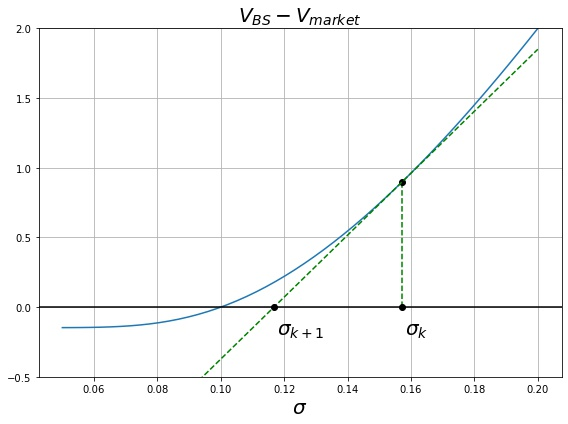
\includegraphics[width=0.65\linewidth]{10_figs/newton.jpg}
        \label{fig:enter-label}
    \end{figure}
}
\end{frame}

\begin{frame}{Модели локальной волатильности}
    \begin{itemize}
        \onslide<1->{\item Пусть динамика процесса задаётся СДУ:
        $$
            \begin{cases} 
            \dfrac{dS_t}{S_t} = r dt + \sigma(t, S_t) dW_t
            \\
            S_0 = s
            \end{cases}
        $$}
        
        \onslide<2->{\item $\sigma(t, S_t)$ -- функция локальной волатильности.}
        \onslide<3->{\item $\sigma(t, S_t) = \sigma(t)$ -- GBM, модель Блэка-Шоулза.}
        \onslide<4->{\item Пример: $\sigma(t, S_t) = \dfrac{\beta}{S_t} \to $
        \begin{align*}
            &dS_t = S_t r dt + \sigma dW_t \\ 
            &S_t = s e^{r t} + \beta \int_0^t e^{r (t-u)} dW_u \sim N(s e^{\mu t}, \ldots)
        \end{align*}}
    \end{itemize}
\end{frame}

\begin{frame}{Уравнение Фоккера-Планка}
    Пусть $dX_t = \mu(t, X_t) dt + \Sigma(t, X_t) dW_t$
    
    \onslide<1->{\begin{block}{Теорема}
        Пусть $h(t, x) = \mathbb{E} \left[ h(T, X_T) | X_t = x \right]$. Тогда:
        $$
              \dfrac{\partial h}{\partial t} + \mu(t, x)\dfrac{\partial h}{\partial x}  + 0.5 \Sigma^2(t, x) \dfrac{\partial^2  h}{\partial x^2} \overset{def}{=} \dfrac{\partial h}{\partial t} + A[h](t, x) = 0    
        $$
    \end{block}}
    
    \onslide<2->{\begin{block}{Теорема}
        Пусть $p(t, x)$ -- плотность процесса $X_t$. Тогда она удовлетворяет уравнению Фоккера-Планка:
        $$
            \dfrac{\partial p}{\partial t} = -\dfrac{\partial}{\partial x} \left[ \mu(t, x) p(t, x) \right] + 0.5 \dfrac{\partial^2}{\partial x^2} \left[ \Sigma^2(t, x) p(t, x) \right] \overset{def}{=} A^*[p](t, x) 
        $$
    \end{block}}
\end{frame}

\begin{frame}{Уравнение Фоккера-Планка}
    \begin{itemize}
        \onslide<1->{\item Пусть $h(t, X)$ -- бесконечно гладкая финитная функция:
        \begin{align*}
            &0=h(T, X_T) = h(0, X_0) + \int_0^T dh(t, X_t) = [\text{Формула Ито}]\\
            &= \int_0^T \left( \dfrac{\partial h}{\partial t} + A[h](t, X_t)\right) dt + \int_0^T \dfrac{\partial h}{\partial X_t} \Sigma(t, X_t) dW_t
        \end{align*}
        где $A[h](t, x) = \mu(t, x) \dfrac{\partial h}{\partial x} + 0.5 \Sigma^2(t, x) \dfrac{\partial^2 h}{\partial x^2}$}

        \onslide<2->{\item Берём слева и справа мат. ожидание:
        \begin{align*}
            &\mathbb{E} \int_0^T dt \left( \dfrac{\partial h}{\partial t} + A[h](t, X_t)\right) dt = \int_0^T dt \mathbb{E} \left( \dfrac{\partial h}{\partial t} + A[h](t, X_t)\right) dt = \\
            &= \int_0^T dt \int_{\mathbb{R}} dx p(t, x)  \left( \dfrac{\partial h}{\partial t} + A[h](t, x)\right) = 0
        \end{align*}}
    \end{itemize}
\end{frame}

\begin{frame}{Уравнение Фоккера-Планка}
    \begin{itemize}
        \item Берём интеграл по частям:
        \onslide<1->{$$
            \int_0^T p(t, x) \dfrac{\partial h}{\partial t} dt = p(t, x) h(t, x)|_{0}^T - \int_0^T h(t, x) \dfrac{\partial p}{\partial t} dt
        $$}
        \onslide<2->{$$
            \int_{\mathbb{R}} p(t, x) \mu(t, x) \dfrac{\partial h}{\partial x}dx = -\int_{\mathbb{R}} h(t, x) \dfrac{\partial}{\partial x} \left[ \mu(t, x) p(t, x) \right] dx
        $$}
        \onslide<3->{$$
            \int_{\mathbb{R}} p(t, x) \Sigma^2(t, x) \dfrac{\partial^2 h}{\partial x^2}dx = \int_{\mathbb{R}} h(t, x) \dfrac{\partial^2}{\partial x^2} \left[ \Sigma^2(t, x) p(t, x) \right] dx
        $$}
        \onslide<4->{Итого:
        $$
            0 = \int_0^T dt \int_{\mathbb{R}} dx h(t, x) \left( -\dfrac{\partial p}{\partial t} + A^*[p](t, x)\right) 
        $$}
        \onslide<5->{\item В силу произвольности функции $h(t, x)$:
        $$
            \dfrac{\partial p}{\partial t} = A^*[p](t, x) \overset{def}{=} -\dfrac{\partial}{\partial x} \left[ \mu(t, x) p(t, x) \right] + 0.5 \dfrac{\partial^2}{\partial x^2} \left[ \Sigma^2(t, x) p(t, x) \right]
        $$}
    \end{itemize}
\end{frame}

\begin{frame}{Формула Дюпира}
    \begin{block}{Формула Дюпира}
        Пусть $\dfrac{dS_t}{S_t} = r dt + \sigma(t, S_t) dW_t$. Тогда цены опционов $C(T, K) = e^{-rT}\mathbb{E} (S_T - K)^+$ удовлетворяют уравнению:
        $$
            \dfrac{\partial C}{\partial T} + rK\dfrac{\partial C}{\partial K} = \dfrac{1}{2} K^2 \sigma^2(T, K) \dfrac{\partial^2 C}{\partial K^2} 
        $$
    \end{block}

    И обратно, если мы в качестве локальной волатильности выберем функцию:
    $$
        \sigma_{loc}^2(t, S) =2 \dfrac{C_T + rKC_K}{K^2 C_{KK} } |_{T=t, K=S}
    $$то попадём в поверхность цен опционов $C(T, K)$. 
\end{frame}


\begin{frame}{Формула Дюпира}
    Док-во для случая $r=0$. 
    \begin{itemize}
    \onslide<1->{\item Пусть $p(t, x)$ -- плотность процесса $S_t$. 
    \begin{align*}
        &\dfrac{\partial C}{\partial T} = \int_{K}^{\infty} (x-K) \dfrac{\partial p(T, x)}{\partial T} dx = \text{[Фоккер-Планк]}\\
        &= \int_K^{\infty} (x-K) A^*[p](T, x) dx = \int_K^{\infty} (x-K)  0.5 \dfrac{\partial^2}{\partial x^2} \left[ x^2 \sigma^2 p \right] dx
    \end{align*}}
    \onslide<2->{
    \item Берём интеграл по частям:
    \begin{align*}
         &\int_K^{\infty} (x-K) \dfrac{\partial^2}{\partial x^2} \left[ x^2 \sigma^2 p \right] dx = -\int_K^{\infty} \dfrac{\partial}{\partial x} \left[ x^2 \sigma^2 p \right] dx  = \sigma^2 K^2 p
    \end{align*}}
    \onslide<3->{\item Из домашки $\dfrac{\partial^2 C}{\partial K^2} = p(T, K)$}
    \onslide<4->{\item Итого:
        $$
            \dfrac{\partial C}{\partial T} = \dfrac{1}{2} K^2 \sigma^2(T, K) \dfrac{\partial^2 C}{\partial K^2} 
        $$}
    \end{itemize}
\end{frame}

\end{document}
